\section{Overview of Results}
This chapter presents interface-level and functional results observed after implementation. The findings confirm that role-based operations, performance analytics, and communication workflows are functioning as intended.

\section{Login Interface}
\begin{figure}[H]
\centering
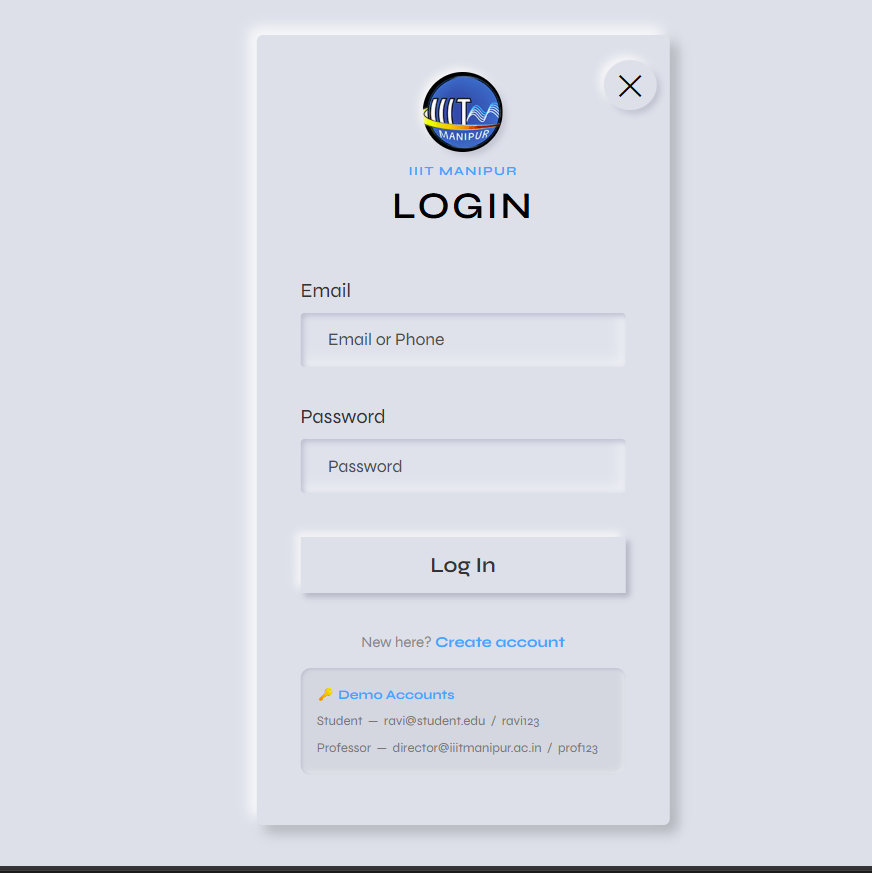
\includegraphics[width=0.9\textwidth]{screenshots/login.png}
\caption{Login Page}
\end{figure}
\noindent\textit{The login interface provides secure access using registered credentials. It acts as the common entry point for all role-based workflows.}

\section{Registration Interface}
\begin{figure}[H]
\centering
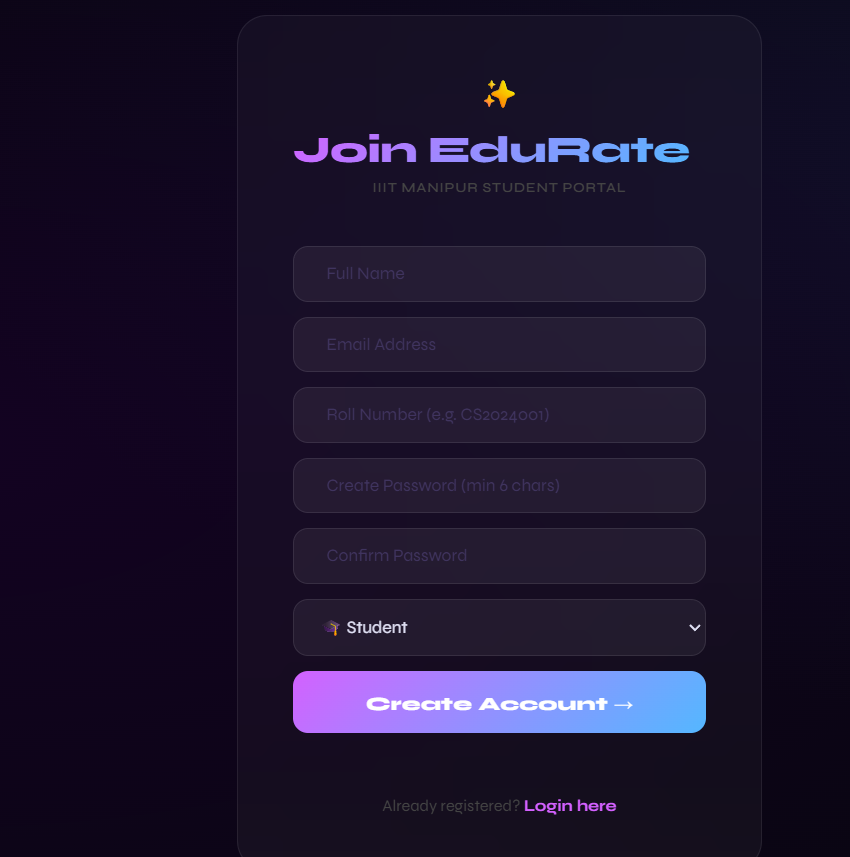
\includegraphics[width=0.9\textwidth]{screenshots/register.png}
\caption{Registration Page}
\end{figure}
\noindent\textit{The registration page captures user details and creates new accounts with role mapping. Input validation ensures completeness and basic data correctness.}

\section{Student Dashboard}
\begin{figure}[H]
\centering
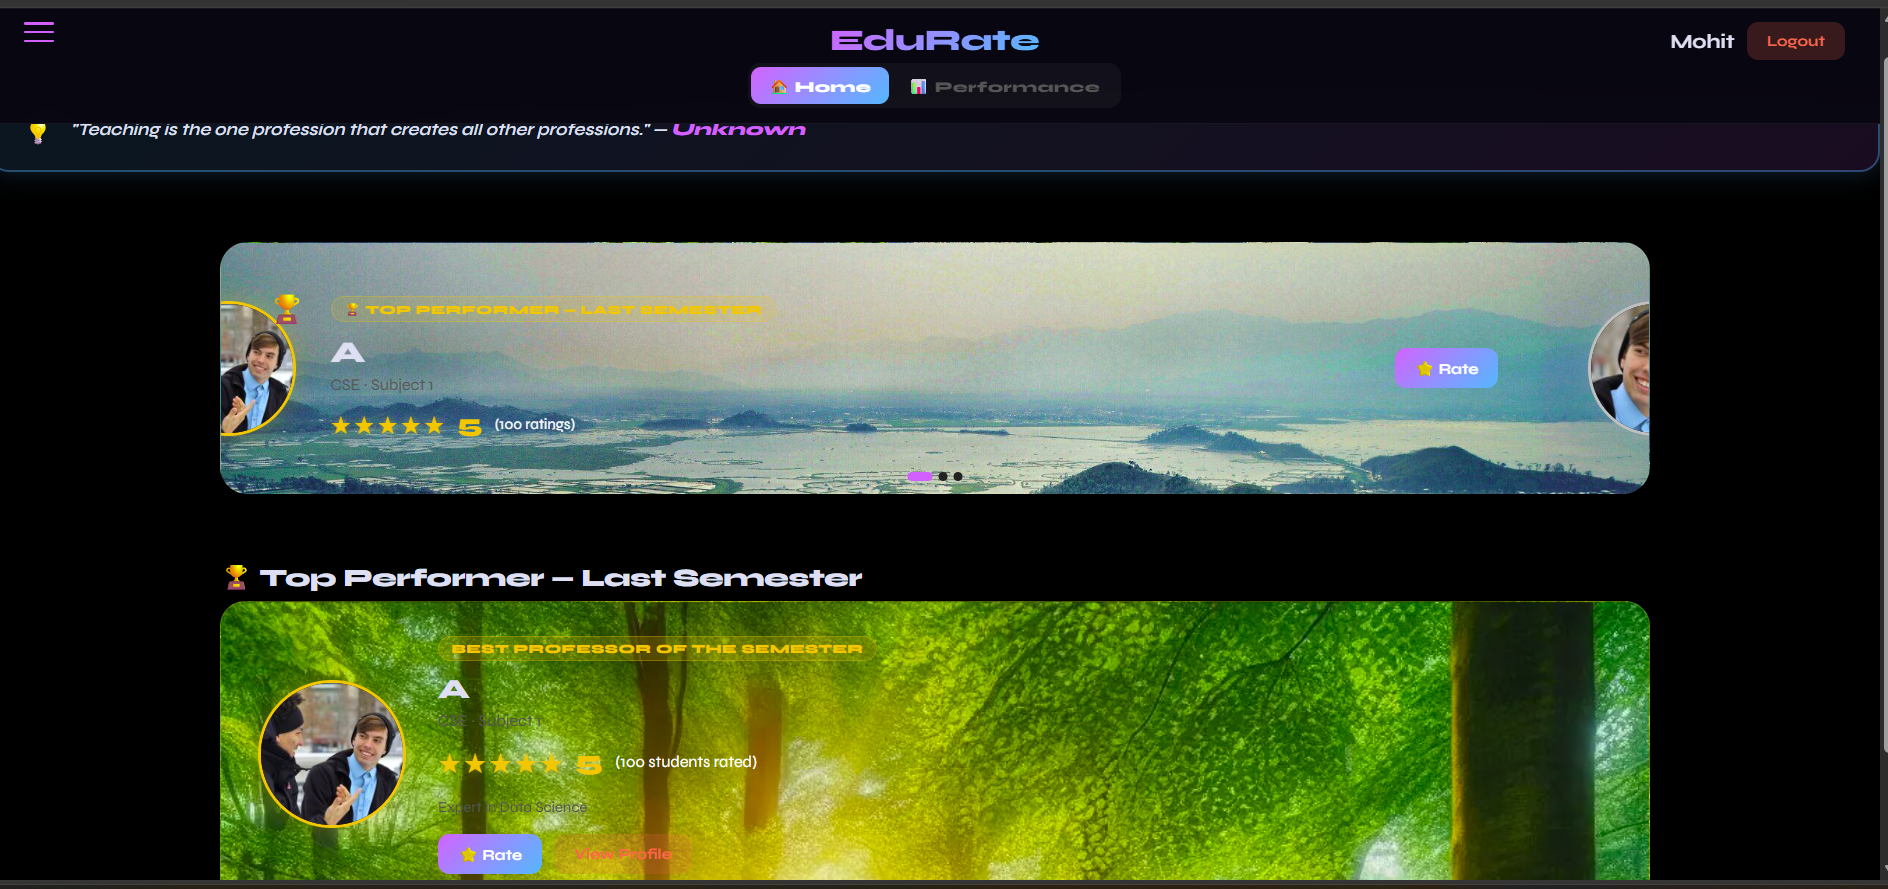
\includegraphics[width=0.95\textwidth]{screenshots/dashboard_student.png}
\caption{Student Dashboard}
\end{figure}
\noindent\textit{The student dashboard consolidates key learning support actions in one place. It offers quick navigation to ratings, doubts, and performance tools.}

\section{Menu Interface}
\begin{figure}[H]
\centering
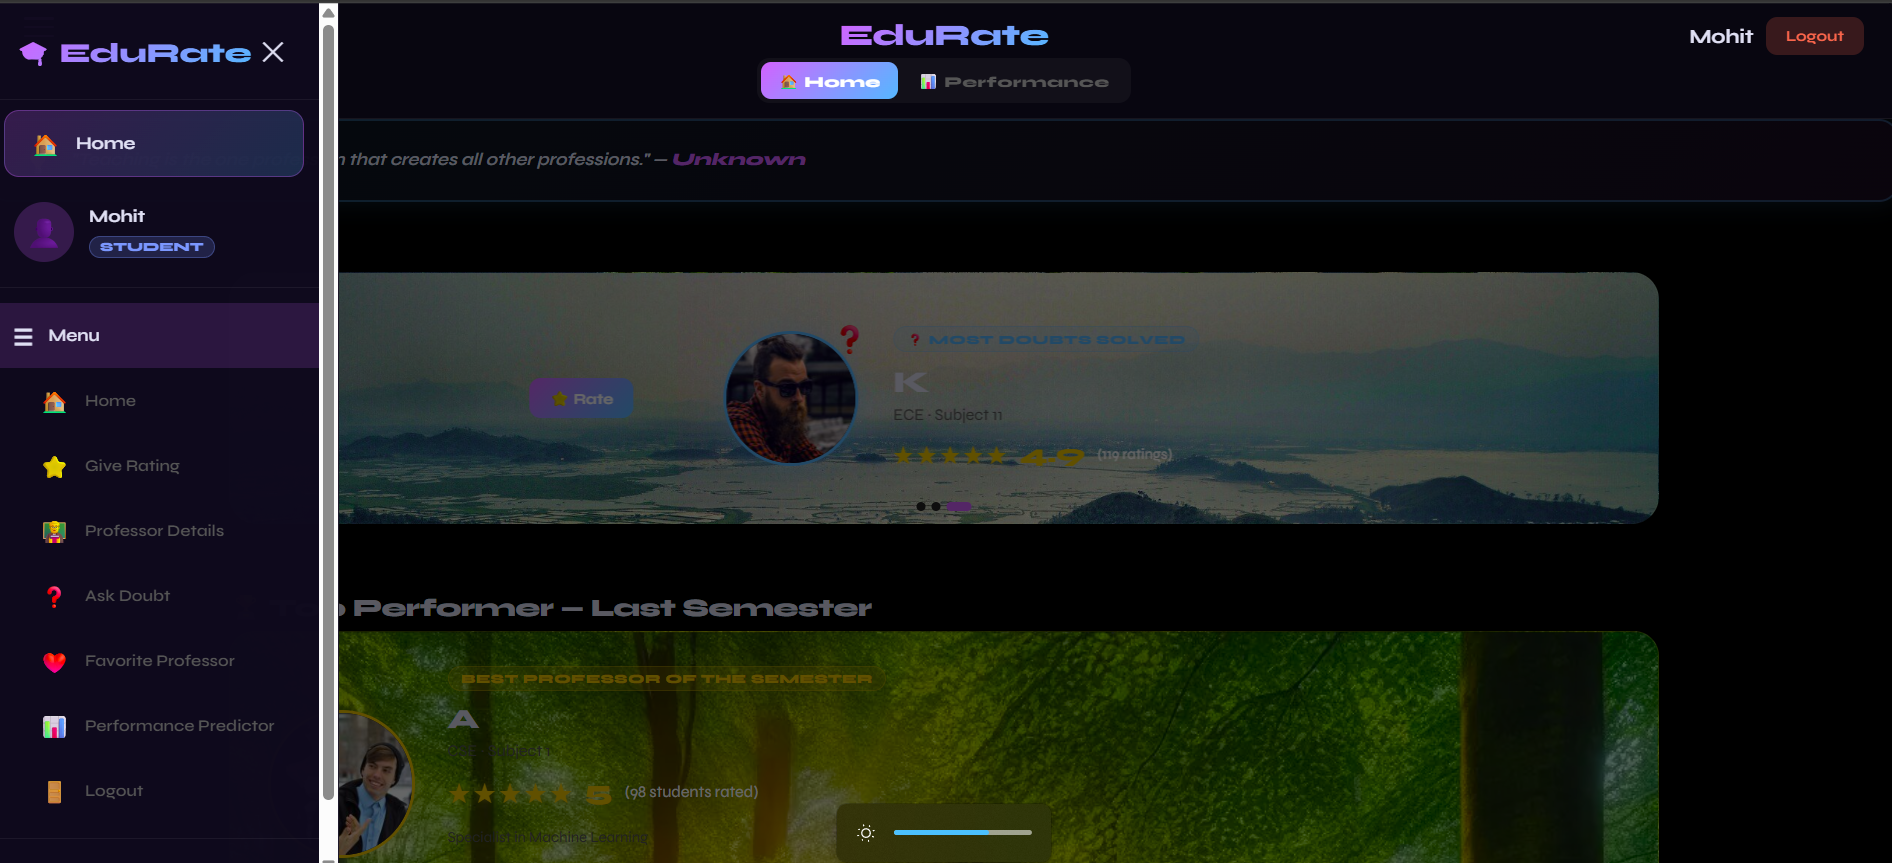
\includegraphics[width=0.95\textwidth]{screenshots/menu.png}
\caption{Dashboard Menu}
\end{figure}
\noindent\textit{The dashboard menu presents organized navigation for role-specific modules. It improves usability by reducing interaction complexity across features.}

\section{Doubt Module}
\begin{figure}[H]
\centering
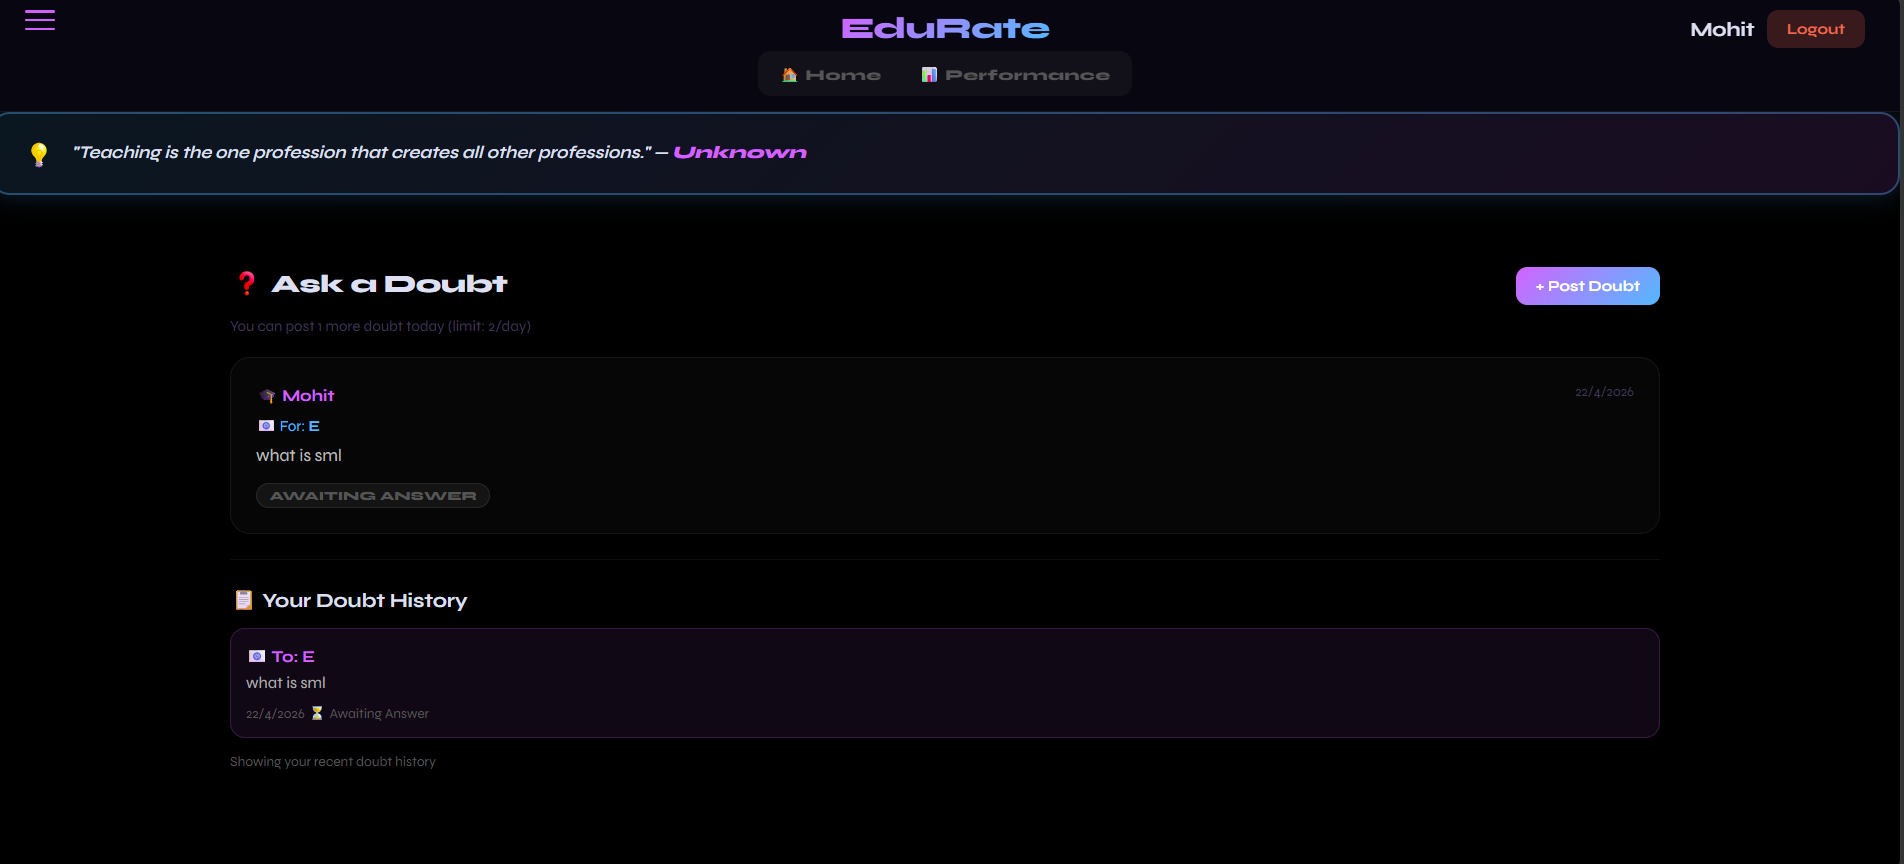
\includegraphics[width=0.95\textwidth]{screenshots/Doubt.png}
\caption{Doubt Posting and Response Module}
\end{figure}
\noindent\textit{This module enables students to post academic queries and receive faculty responses. Daily constraints and status visibility maintain structured interaction.}

\section{Performance Predictor Form}
\begin{figure}[H]
\centering
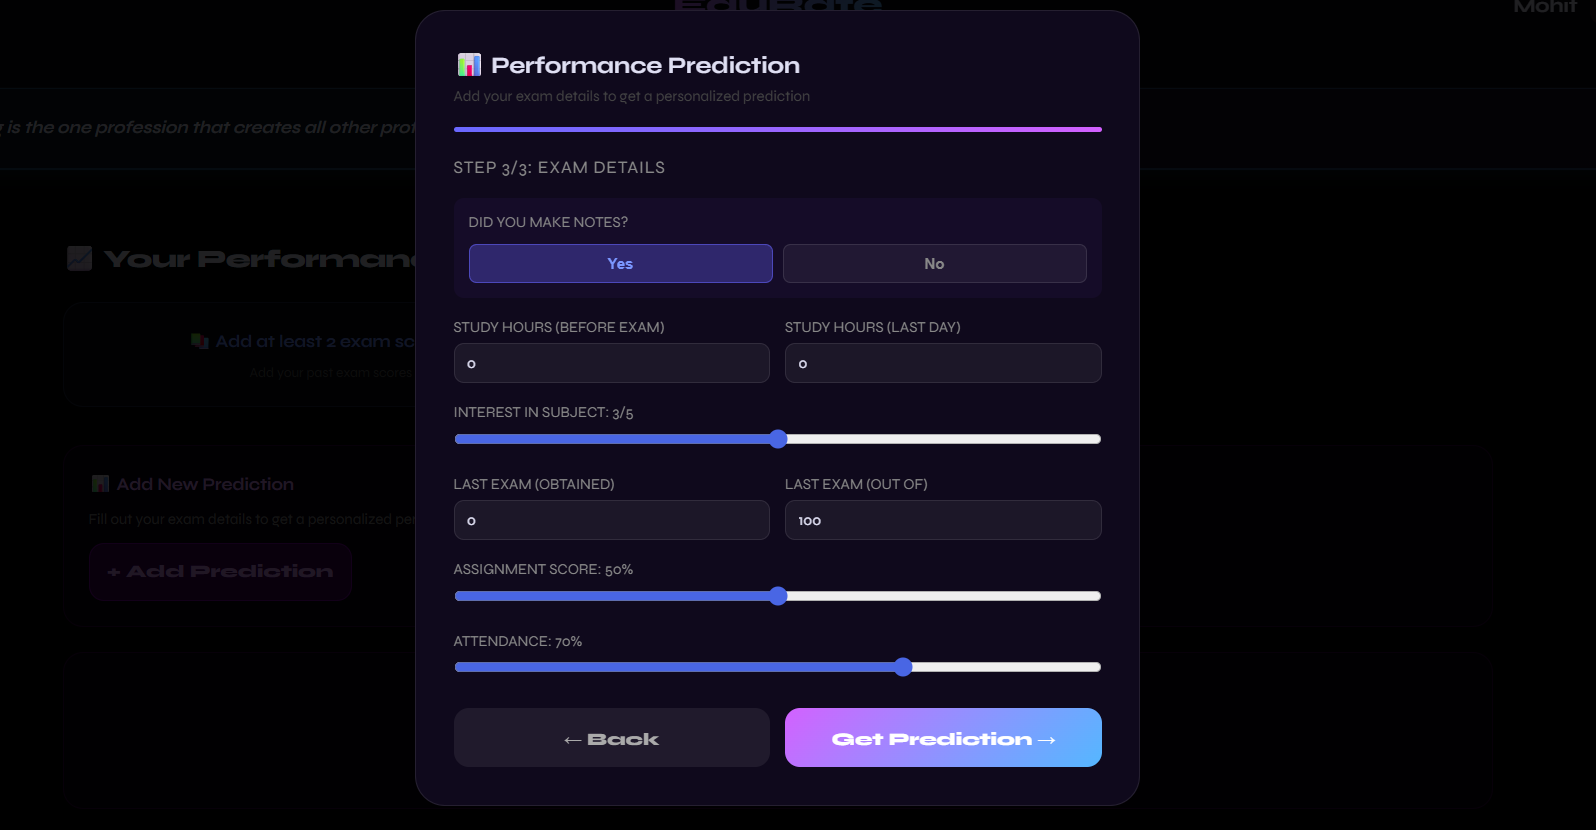
\includegraphics[width=0.95\textwidth]{screenshots/performance_prediction.png}
\caption{Performance Prediction Input Form}
\end{figure}
\noindent\textit{The prediction form collects multi-factor study and assessment inputs. These values are used to estimate expected academic performance.}

\section{Prediction Output}
\begin{figure}[H]
\centering
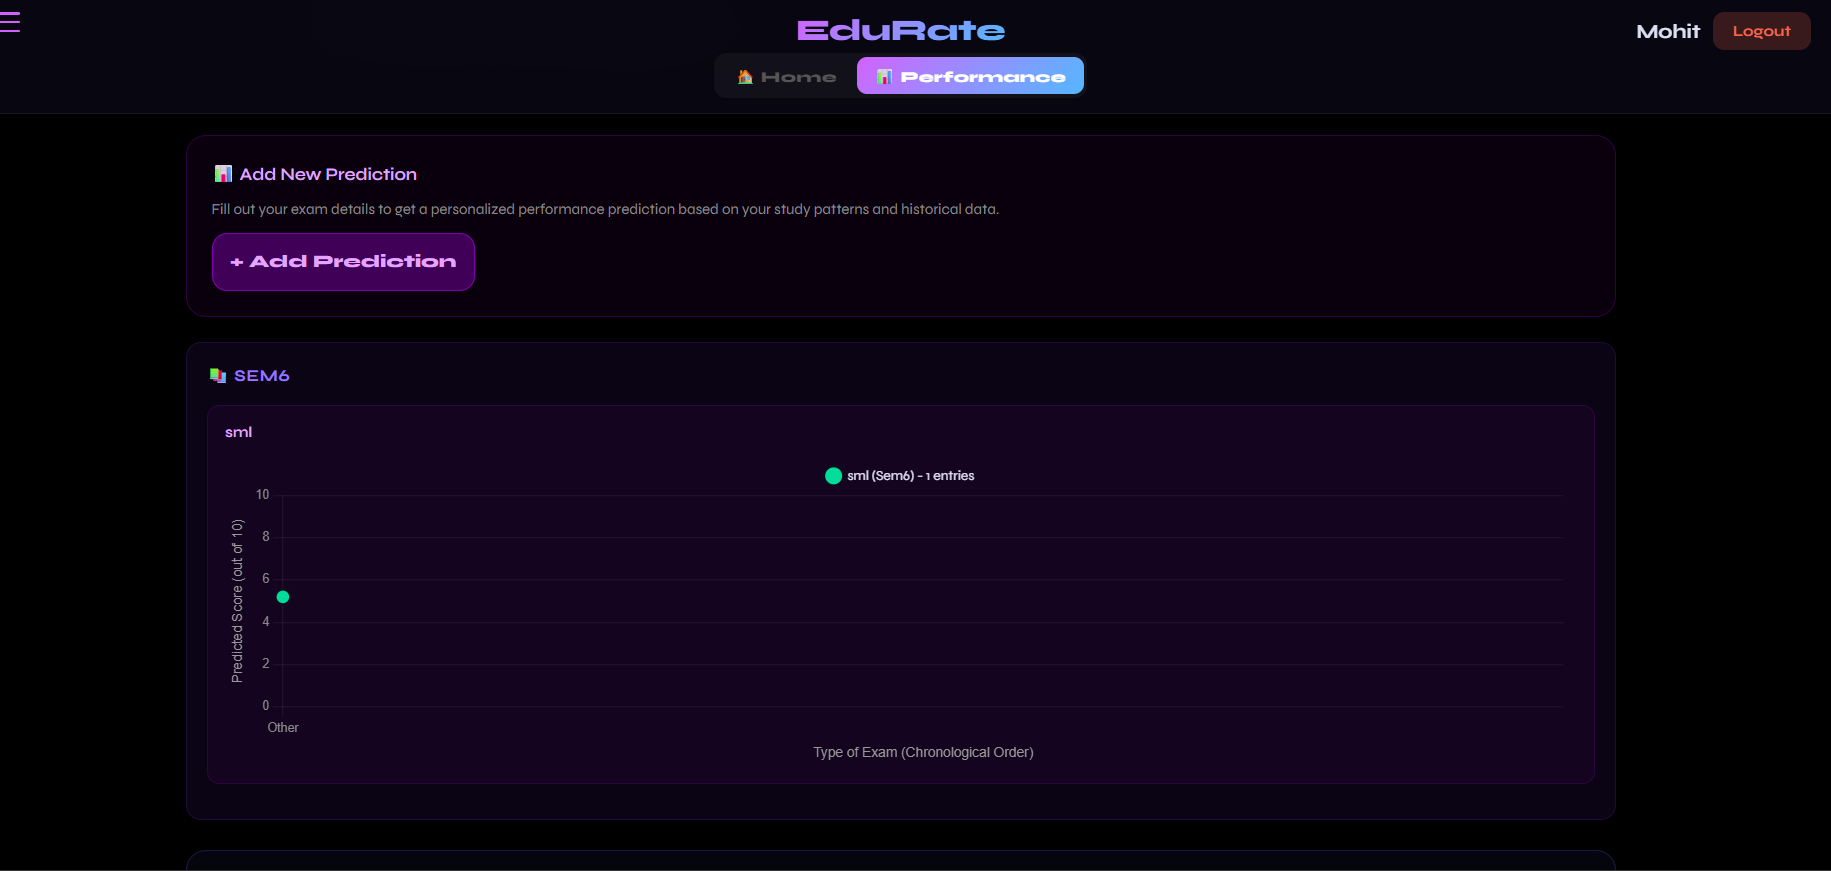
\includegraphics[width=0.95\textwidth]{screenshots/after_prediction.png}
\caption{Performance Prediction Result}
\end{figure}
\noindent\textit{The result screen displays expected score and interpretation after processing inputs. It supports quick feedback for improving preparation strategies.}

\section{Admin Dashboard}
\begin{figure}[H]
\centering
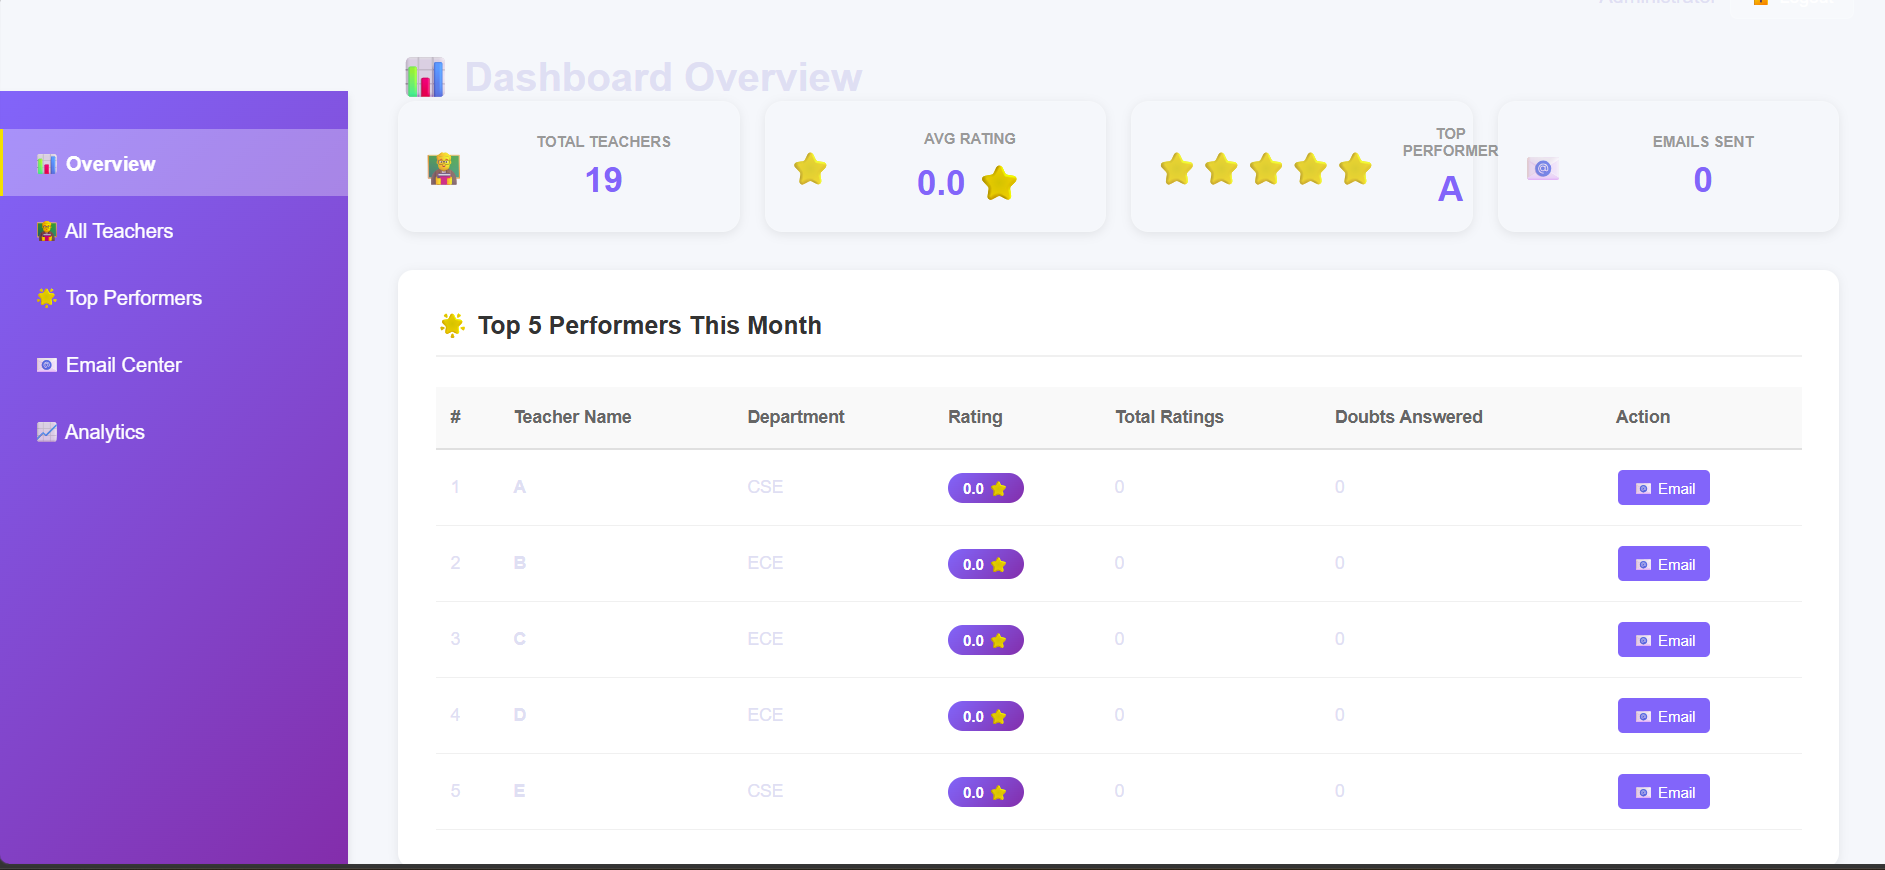
\includegraphics[width=0.95\textwidth]{screenshots/Admin-Dashboard.png}
\caption{Admin Dashboard with Analytics}
\end{figure}
\noindent\textit{The admin dashboard provides institutional-level performance monitoring. It integrates rankings, summary metrics, and communication controls for reporting.}

\section{Observed Results}
\begin{enumerate}[label=\Alph*., leftmargin=1.5em]
    \item Student feedback collection and professor rating functions operate correctly.
    \item Doubt posting constraints and response flow are operational.
    \item Prediction history and chart visualization are updated dynamically.
    \item Admin performance monitoring and email reporting are integrated.
\end{enumerate}

\section{Core Functional Outcomes}
\begin{enumerate}[label=\Alph*., leftmargin=1.5em]
    \item \textbf{Authentication:} Role-based redirection works reliably for all user categories.
    \item \textbf{Rating Workflow:} Professor-wise rating aggregation updates correctly after submissions.
    \item \textbf{Doubt Workflow:} Student-to-professor query lifecycle is completed with status visibility.
    \item \textbf{Prediction Module:} Multi-factor input successfully generates expected score output and trend records.
    \item \textbf{Admin Analytics:} Teacher performance ranking and bulk communication are operational.
\end{enumerate}

\section{Technical Achievement Highlights}
\begin{enumerate}[label=\Alph*., leftmargin=1.5em]
    \item Integration of frontend and backend modules with consistent role checks.
    \item Combined chart visualization with persisted prediction data.
    \item Reporting automation through email APIs.
    \item Readable and modular code organization for maintainability.
\end{enumerate}

\section*{Chapter Summary}
This chapter demonstrated the implementation outcomes through interface evidence, workflow verification, and functional observations. The presented screenshots and explanations confirm that the system behaves correctly across student, professor, and admin roles.
